\documentclass{article}
\usepackage[utf8]{inputenc}
\usepackage{graphicx}
\graphicspath{ {images/} }

\title{Results/Discussion}
\author{pwang16 }
\date{April 2016}

\begin{document}

\maketitle

\section{Satellite Change}
Throughout the simulation, 3 different types of satellites around the Milky Way were modeled, described in the table below:

\begin{center}
	\begin{tabular}{| l | l | l | l | }
		\hline Satellite & $M/M_{mw, vir}$ & $R/R_{mw, vir}$ & $V_{max}/V_{mw, max}$ \\ \hline
		Massive & $1.9 \times 10^{-2}$ & $9.02 \times 10^{-2}$ & 0.45 \\ \hline
		Sagittarius & $9.0 \times 10^{-4}$ & $3.38 \times 10^{-2}$ & 0.16 \\ \hline
		Small & $9.9 \times 10^{-5}$ & $1.66 \times 10^{-2}$ & 0.08 \\ \hline
	\end{tabular}
\end{center}

As the satellite's gravity increases as the mass changes, the stellar streams produced in this interaction would be subject to the same change. By starting out the massive satellite as an isotropic ball of mass and evolving it along a circular orbit with $r = 0.4R_{vir}$, it was found that the satellite produced a stellar stream unlike initially expected. Originally, it was predicted that the stellar stream would trace along the orbital path, leaving behind trails of stars that would eventually be swept up again once the satellite passed by that area of the orbit. In this manner, enough stars would eventually leak from the satellite and form a secondary stellar stream ring around the orbit. However, it was found that the satellite produced a stellar stream with two distinctive parts: a leading tail that quickly fell into the center of the Milky Way, and also created a smaller trailing tail. This is extremely similar to the results found by Choi et al. (2008) \cite{dymanicsOfTidalTails}, who found that the leading tail tilts towards the center of the halo (akin to the Milky Way used in our simulation), and had a trailing tail that is distributed outside the orbital radius. While the tail modeled by Choi et al. started to point directly towards the center of the halo, the tail I found did not. This suggests that possibly more time should be allotted for the simulation, as Choi's leading tail only began to point towards the center at late times. In both cases, stars within the leading tail were found to lose energy and angular momentum, resulting in their infall into the Milky Way, whereas the orbits in the trailing tail gained energy and angular momentum, leading to the spread of the trailing tail outside the orbit. This can easily be seen within figure 1 from Choi et al, where the differences in energy are clear within the orbital rotation. 

\begin{figure}
	\centering
	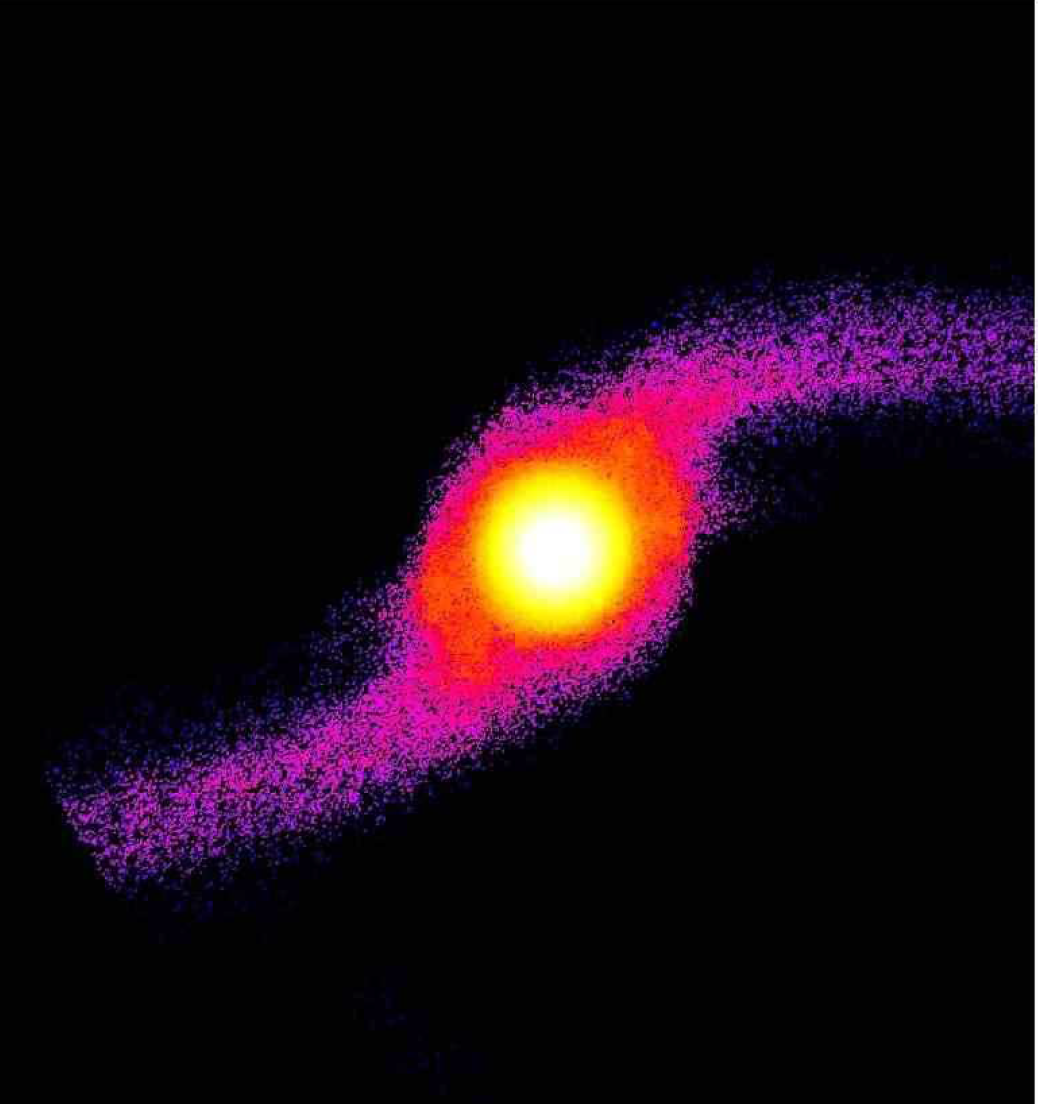
\includegraphics[width=0.5\textwidth]{tailStreams}	
	\caption{The tail streams of a satellite, from Choi et al. (2008)}
\end{figure}

The tail morphology for both the Sagittarius and small sized satellites correspond in the same manner, with the leading tail moving inwards towards the Milky Way and the trailing tail moving outside the orbital radius, eventually becoming smeared along the orbital path. A minor detail in tail morphology for the Sagittarius and small sized satellites is that their tails exhibit major angular shifts in their leading tails. While the large satellite falls changes into a spiral fashion (``S'' shape), the Sagittarius and small sized satellites exhibit much sharper turns instead of curving into the center of the Milky Way (``Z'' shape). This is explained by Johnston et al. (2001) \cite{debrisSatellite}, where the sharp angles are a result of the epicyclic motion of the tails alongside the satellite being accelerated at subsequent apocenters. The first sharp turn correlates with the first apocenter of the ejecta, which suggests that the deceleration during escape causes these sharp turns to occur. Choi et al. \cite{binneyTremaine} suggest using a three-body approach to understanding these orbits, using a conserved Jacobi constant with:

\[
E_J = E - \Omega^{\rightarrow}_{s}\cdot L^{\rightarrow} 
\]

where $E$ is the orbital energy, $L^{\rightarrow}$ is the angular momentum, and $\Omega^{\rightarrow}_s$ is the angular frequency of the satellite around the Milky Way. Since the strength of the inversion symmetry around the satellite is inversely proportional to the satellite mass \cite{dymanicsOfTidalTails}, small satellites have a tidal force that is symmetric around the center of the satellite, which then leads to symmetric masses within the leading and trailing tails. In large satellites, however, the asymmetric tidal force means the leading and trailing tails are asymmetric themselves. 

\section{Discussion}
``S'' and ``Z'' shape tails have already been previously observed by Grillmair \& Dionatos (2006) \cite{grillmairDionatos} and Leon \& Combes (2000) \cite{leonCombes}, which suggests that the simulations carried out are correct representations. However, due to the simplicity of the simulations carried out, the results are not wholly correct. The simulation only takes into account the two theorized dynamical principles that affect stellar stream production \cite{ringsAndPseudoRings}: 1) the leading and trailing points where the attractive force of the host galaxy and the satellite are equal and divergent, leading to a balance at zero velocity, and 2) the escaping stars that form the stellar stream are affected differently for the leading and trailing stream, with the leading stream being decelerated and the trailing stream being accelerated from the original orbital spot. Choi et al. \cite{dymanicsOfTidalTails} showed that these two dynamical principles are consistant with the effect of the satellite's self gravitational force on the tail is only weakly related to the satellite's mass, which then means that the acceleration on the satellite after escapes begins to have a significant effect for satellites with masses greater than or equal to the mass of the Sagittarius galaxy. 

Due to this, the simulations imply that any satellite will create a stellar stream that is displaced from the original orbital position. The direction, shape, and magnitude of displacement are all related to the satellite mass, with higher mass satellites causing larger, thicker, and less tightly bound stellar streams. Furthermore, the velocity distribution of the massive satellite during the creation of the stellar stream is scattered isotropically between stars ejected. 

To complete the simulation, there were some major assumptions made about the initial conditions. First, the effects of dynamical friction were completely ignored, as Chandrasekhar (1943) found that dynamical friction was only relevant on a star's nearest neighbors \cite{dynamicalFriction}. Second, the Milky Way halo was modeled to be completely isotropic and spherical, which affected the models of the satellites. If the Milky Way halo was properly modeled, the stellar streams created would exhibit greater changes along different parts of the Milky Way. Third, the satellite was assumed to be on a circular orbit around the Milky Way well within the tidal disruption radius of the Milky Way. If proper tidal movements were carried out and modeled as the satellite galaxy moved closer to the Milky Way, the stellar stream created would exhibit velocity distributions with far more disparities. Finally, the assumption was made that the Milky Way halo remains spherically isotropic despite interactions with the satellite, that is, only the satellite would create the stellar stream. Properly speaking, stars from the Milky Way would also be pulled out of orbit in order to create the stellar stream, but those stars are far less numerous than the stars from the satellite. In spite of these assumptions, I felt the simulations accurately explored the most important factor relating to stellar stream creation: the mass of the satellite galaxy. 



\bibliography{results} 
\bibliographystyle{unsrt} \end{document}